\documentclass{beamer}

\usetheme[secheader]{Boadilla}
\usecolortheme{beetle}
\usepackage[latin1]{inputenc}

\title{Forgetting the C in C++}
\author{Alexander Kondratskiy}
\date{\today}
% \institute[2008]{ECON 101}

\begin{document}

\frame{\titlepage}

\section{Introduction}

\frame {
	\frametitle{What is he talking about?}
	\begin{itemize}
        \item<2->Overview of C++, from a C programmer's perspective
        \item<2->Good C++ coding style
        \item<2->More than "C with classes"
        \item<2->Fixing bad habbits learnt from C.
	\end{itemize}
}

\frame {
	\frametitle{Why is he talking about it?}
	\begin{itemize}
        \item<1->C++ has evolved
        \item<2->Safety (less memory management, type safety)
        \item<3->Readability/maintainability
        \begin{quote}<3->
"Programs must be written for people to read, and only incidentally for machines to execute."
-Abelson/Sussman, SICP
        \end{quote}
        \item<4->Programmer productivity (STL, abstractions)
        \item<5->Efficiency and speed (providing context for compiler)
        \item<5->Win-win
	\end{itemize}
}

\frame {
	\frametitle{How will we do it?}
	\begin{itemize}
		\item<1->Observe common C idiom
		\item<1->Why it's "bad" in C++
		\item<1->C++ alternative
		\item<1->Gains from the alternative
		\item<2->Learn new techniques/features along the way
	\end{itemize}
}

\section{Prerequisites}

\frame {
	\frametitle{History of C++}
	\begin{itemize}
        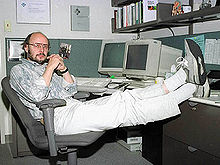
\includegraphics[height=2cm]{220px-BjarneStroustrup.jpg}
    \end{itemize}
}

\end{document}
